\documentclass[border=2pt]{standalone}
\usepackage{amsmath}
\usepackage{tikz}
\usetikzlibrary{arrows.meta,shapes.symbols}
\begin{document}
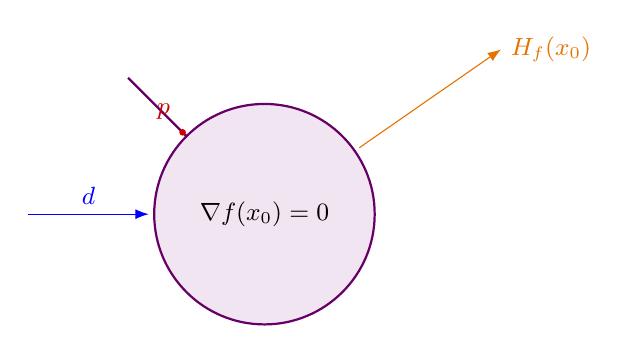
\begin{tikzpicture}[>=Latex,every node/.style={font=\small}]
  \node[shape=magnifying glass,draw=violet!80!black,fill=violet!10,thick,
    minimum size=28mm,outer sep=2pt,magnifying glass handle angle=135,
    magnifying glass handle aspect=.75] (critical)
    {$\nabla f(x_0)=0$};
  \draw[->,blue] (-3,0) -- (critical)
    node[midway,above] {$d$};
  \draw[->,orange!90!black] (critical.35) -- ++(1.8,1.25)
    node[right] {$H_f(x_0)$};
  \fill[red!80!black] (critical.north west) circle (1.2pt)
    node[above left=1pt] {$p$};
\end{tikzpicture}
\end{document}
